\documentclass{standalone}
\usepackage{tikz}
\usetikzlibrary{patterns}
\usetikzlibrary{positioning}
\usetikzlibrary{patterns, positioning}
\usetikzlibrary{shapes.misc}
\usepackage[outline]{contour}
\contourlength{1.5pt} 
\usepackage[sfdefault]{ClearSans}

\begin{document}
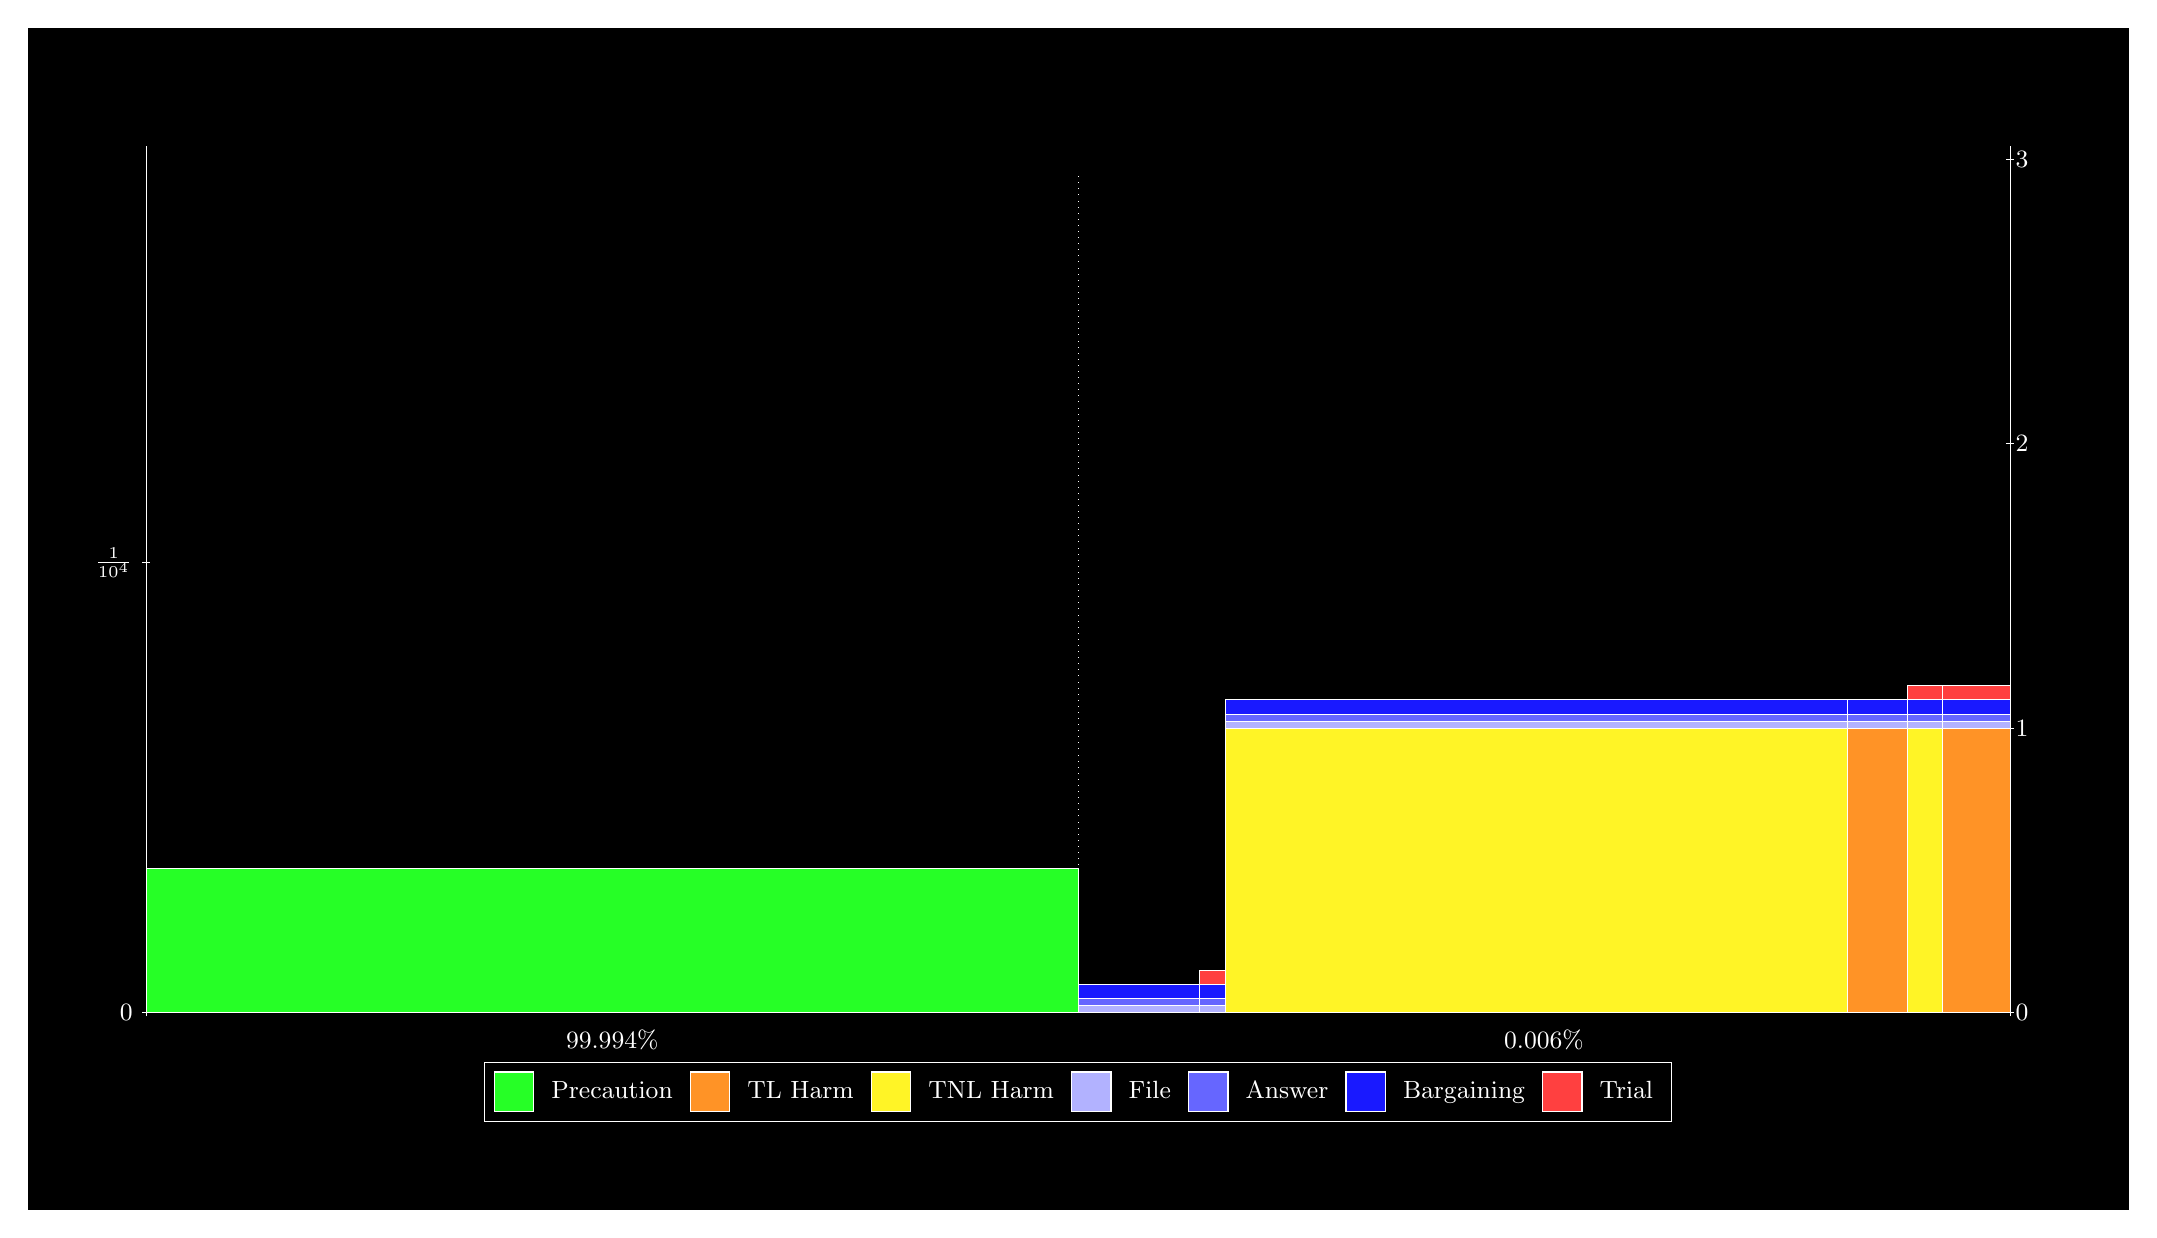
\begin{tikzpicture}
\draw[fill=black] (0,0) rectangle (26.667,15);
\draw[fill=green!85,draw=white,very thin] (1.5,2.5) rectangle (13.333,4.3285);
\draw[fill=green!85,draw=white,very thin] (13.333,2.5) rectangle (14.876,2.5001);
\draw[fill=blue!30,draw=white,very thin] (13.333,2.5001) rectangle (14.876,2.5904);
\draw[fill=blue!60,draw=white,very thin] (13.333,2.5904) rectangle (14.876,2.6807);
\draw[fill=blue!90,draw=white,very thin] (13.333,2.6807) rectangle (14.876,2.8613);
\draw[fill=green!85,draw=white,very thin] (14.876,2.5) rectangle (15.205,2.5001);
\draw[fill=blue!30,draw=white,very thin] (14.876,2.5001) rectangle (15.205,2.5904);
\draw[fill=blue!60,draw=white,very thin] (14.876,2.5904) rectangle (15.205,2.6807);
\draw[fill=blue!90,draw=white,very thin] (14.876,2.6807) rectangle (15.205,2.8613);
\draw[fill=red!75,draw=white,very thin] (14.876,2.8613) rectangle (15.205,3.0419);
\draw[fill=green!85,draw=white,very thin] (15.205,2.5) rectangle (23.103,2.5001);
\draw[fill=yellow!85,draw=white,very thin] (15.205,2.5001) rectangle (23.103,6.112);
\draw[fill=blue!30,draw=white,very thin] (15.205,6.112) rectangle (23.103,6.2023);
\draw[fill=blue!60,draw=white,very thin] (15.205,6.2023) rectangle (23.103,6.2926);
\draw[fill=blue!90,draw=white,very thin] (15.205,6.2926) rectangle (23.103,6.4732);
\draw[fill=green!85,draw=white,very thin] (23.103,2.5) rectangle (23.866,2.5001);
\draw[fill=orange!85,draw=white,very thin] (23.103,2.5001) rectangle (23.866,6.112);
\draw[fill=blue!30,draw=white,very thin] (23.103,6.112) rectangle (23.866,6.2023);
\draw[fill=blue!60,draw=white,very thin] (23.103,6.2023) rectangle (23.866,6.2926);
\draw[fill=blue!90,draw=white,very thin] (23.103,6.2926) rectangle (23.866,6.4732);
\draw[fill=green!85,draw=white,very thin] (23.866,2.5) rectangle (24.311,2.5001);
\draw[fill=yellow!85,draw=white,very thin] (23.866,2.5001) rectangle (24.311,6.112);
\draw[fill=blue!30,draw=white,very thin] (23.866,6.112) rectangle (24.311,6.2023);
\draw[fill=blue!60,draw=white,very thin] (23.866,6.2023) rectangle (24.311,6.2926);
\draw[fill=blue!90,draw=white,very thin] (23.866,6.2926) rectangle (24.311,6.4732);
\draw[fill=red!75,draw=white,very thin] (23.866,6.4732) rectangle (24.311,6.6538);
\draw[fill=green!85,draw=white,very thin] (24.311,2.5) rectangle (25.167,2.5001);
\draw[fill=orange!85,draw=white,very thin] (24.311,2.5001) rectangle (25.167,6.112);
\draw[fill=blue!30,draw=white,very thin] (24.311,6.112) rectangle (25.167,6.2023);
\draw[fill=blue!60,draw=white,very thin] (24.311,6.2023) rectangle (25.167,6.2926);
\draw[fill=blue!90,draw=white,very thin] (24.311,6.2926) rectangle (25.167,6.4732);
\draw[fill=red!75,draw=white,very thin] (24.311,6.4732) rectangle (25.167,6.6538);
\draw[white,very thin] (1.5,2.5) -- (1.5,13.5);
\draw[white,very thin] (1.45,2.5) -- (1.55,2.5);
\node[font=\small,text=white, anchor=east] at (1.45, 2.5) {0};
\draw[white,very thin] (1.45,8.214) -- (1.55,8.214);
\node[font=\small,text=white, anchor=east] at (1.45, 8.214) {$\frac{1}{10^{4}}$};

\draw[white,dotted,very thin] (13.333,2.83) -- (13.333,13.17);
\draw[white,very thin] (25.167,2.5) -- (25.167,13.5);
\draw[white,very thin] (25.117,2.5) -- (25.217,2.5);
\node[font=\small,text=white, anchor=west] at (25.117, 2.5) {0};
\draw[white,very thin] (25.117,6.1119) -- (25.217,6.1119);
\node[font=\small,text=white, anchor=west] at (25.117, 6.1119) {1};
\draw[white,very thin] (25.117,9.7237) -- (25.217,9.7237);
\node[font=\small,text=white, anchor=west] at (25.117, 9.7237) {2};
\draw[white,very thin] (25.117,13.336) -- (25.217,13.336);
\node[font=\small,text=white, anchor=west] at (25.117, 13.336) {3};

\draw[white,very thin] (1.5,2.5) -- (25.167,2.5);
\draw[white,very thin] (1.5,2.45) -- (1.5,2.55);
\node[font=\small,text=white, anchor=north] at (1.5, 2.45) {};
\draw[white,very thin] (25.167,2.45) -- (25.167,2.55);
\node[font=\small,text=white, anchor=north] at (25.167, 2.45) {};

\node[font=\small,text=white,anchor=south] at (7.4167, 1.9) {99.994\%};
\node[font=\small,text=white,anchor=south] at (19.25, 1.9) {0.006\%};
\draw (13.3333,2.5) node (B) {};
\begin{scope}[align=center]
\matrix[scale=0.5,draw=white,below=0.5cm of B,nodes={draw},column sep=0.1cm]{
\node[rectangle,draw,minimum width=0.5cm,minimum height=0.5cm,fill=green!85]{}; & \node[draw=none,font=\small,text=white]{Precaution}; &
\node[rectangle,draw,minimum width=0.5cm,minimum height=0.5cm,fill=orange!85]{}; & \node[draw=none,font=\small,text=white]{TL Harm}; &
\node[rectangle,draw,minimum width=0.5cm,minimum height=0.5cm,fill=yellow!85]{}; & \node[draw=none,font=\small,text=white]{TNL Harm}; &
\node[rectangle,draw,minimum width=0.5cm,minimum height=0.5cm,fill=blue!30]{}; & \node[draw=none,font=\small,text=white]{File}; &
\node[rectangle,draw,minimum width=0.5cm,minimum height=0.5cm,fill=blue!60]{}; & \node[draw=none,font=\small,text=white]{Answer}; &
\node[rectangle,draw,minimum width=0.5cm,minimum height=0.5cm,fill=blue!90]{}; & \node[draw=none,font=\small,text=white]{Bargaining}; &
\node[rectangle,draw,minimum width=0.5cm,minimum height=0.5cm,fill=red!75]{}; & \node[draw=none,font=\small,text=white]{Trial}; \\\\
};\end{scope}

\end{tikzpicture}
\end{document}